%% Honest submission draft aligned with the released implementation and audited results.
\documentclass[preprint,12pt]{elsarticle}

\usepackage{amssymb}
\usepackage{amsmath}
\usepackage{graphicx}
\usepackage{booktabs}
\usepackage{array}
\usepackage{multirow}
\usepackage{xcolor}
\usepackage[hidelinks]{hyperref}
\usepackage{placeins}

\journal{Journal of Visual Communication and Image Representation}

\begin{document}

\begin{frontmatter}

\title{TextConsistency: Parameter-Free Probability Fusion of Learned Prompts and Class Descriptions for Base-to-Novel Recognition}

\author[1]{Author Name\corref{cor1}}
\ead{author-email@university.edu}
\cortext[cor1]{Corresponding author}

\author[1]{Advisor Name}
\ead{advisor-email@university.edu}

\affiliation[1]{organization={School of XXX, XXX University},
                addressline={XXX Street},
                city={XXX},
                postcode={000000},
                country={China}}

\begin{abstract}
Prompt learning efficiently adapts vision-language models to downstream recognition tasks, but prompts trained on base classes can lose part of the semantic coverage inherited from the frozen model. We study a simple way to recover this coverage without adding trainable parameters. TextConsistency combines the posterior produced by a CoOp prompt with a second posterior obtained from frozen, class-specific natural-language descriptions. Description embeddings are averaged within each class, both branches share the frozen CLIP image encoder, and their class probabilities are fused with a fixed weight of 0.5. The description branch is pre-computed and does not change prompt training.

We evaluate the method with CLIP ViT-B/16 under the 16-shot base-to-novel protocol on ten datasets and three random seeds. TextConsistency obtains an average harmonic mean of 78.75, compared with 75.33 for the matched CoOp runs and 76.15 for locally evaluated CoCoOp. It improves the harmonic mean over CoOp in all 30 seed-level comparisons and over CoCoOp on all ten datasets. Its ten-dataset average is comparable to the published MaPLe result, while remaining 1.59 percentage points below PromptSRC. On an RTX 4090, the fused predictor adds no trainable parameters and increases batch-64 inference latency by 0.74\%. These results show that fixed probability fusion is a practical way to combine task adaptation with frozen semantic priors, although the current study does not include ImageNet and therefore does not establish an eleven-dataset state of the art.
\end{abstract}

\begin{keyword}
vision-language models \sep prompt learning \sep few-shot classification \sep base-to-novel generalization \sep class descriptions \sep probability fusion
\end{keyword}

\end{frontmatter}

\section{Introduction}
\label{sec:introduction}

Large vision-language models such as CLIP and ALIGN learn shared representations from large image-text corpora and support open-vocabulary recognition through textual prompts \cite{radford2021clip,jia2021align}. LiT further shows that a locked image encoder can retain strong visual representations while the text tower is adapted for zero-shot transfer \cite{zhai2022lit}. This transfer ability has motivated parameter-efficient adaptation methods that keep the encoders frozen and optimise only a small prompt. CoOp replaces hand-written context words with continuous learnable vectors and substantially improves few-shot recognition on downstream datasets \cite{zhou2022coop}. The gain on seen classes, however, can be accompanied by weaker transfer to unseen classes. CoCoOp addresses this issue with image-conditioned prompts \cite{zhou2022cocoop}, while later methods introduce prompt distributions, coupled visual-text prompts, knowledge guidance, self-regularisation, or residual classifiers \cite{lu2022proda,khattak2023maple,yao2023kgcoop,khattak2023promptsrc,yu2023taskres}.

Learned prompts and descriptive language provide different information. A learned context adapts efficiently to the labelled base samples, whereas natural-language descriptions retain explicit attributes, parts, scenes, and functions. CuPL demonstrates that class-specific descriptions generated by a language model can improve zero-shot recognition \cite{pratt2023cupl}. In our experiments, the frozen description branch alone does not outperform CoOp on average, but its errors are sufficiently complementary to improve base-to-novel balance when the two predictions are combined.

This observation motivates TextConsistency, a deliberately small extension to prompt learning. For each class, we encode a fixed collection of natural-language descriptions with the frozen CLIP text encoder, average their normalised embeddings, and normalise the resulting class prototype. At inference, we compute one posterior from the learned CoOp prompt and one from the frozen description prototype. The final posterior is their arithmetic mean. We fix the mixing coefficient to 0.5 for every dataset and do not tune a temperature, gate, threshold, or class-specific weight.

The simplicity of the method is useful for two reasons. First, it isolates the value of semantic complementarity from gains produced by a larger trainable architecture. Second, the description embeddings can be cached, so the method adds no trainable parameters and only a small matrix multiplication and probability average at inference. This is particularly suitable when the goal is to improve novel-class transfer while preserving the efficient training procedure of CoOp.

The contributions of this paper are as follows:
\begin{itemize}
    \item We introduce a fixed probability-fusion formulation that combines a learned prompt posterior with a frozen class-description posterior. It uses the existing CLIP encoders and adds no trainable parameters beyond CoOp.
    \item We provide controlled component and class-name studies that separate branch complementarity from ordinary class-name ensembling. Across all ten datasets with matched checkpoints, descriptions add 1.53 HM points over class-name fusion.
    \item We evaluate the same 0.5 fusion rule on ten base-to-novel datasets. TextConsistency reaches 78.75 average HM, improves over local CoCoOp on ten out of ten datasets, and improves over matched CoOp in all 30 seed-level comparisons.
    \item We report measured inference cost on one RTX 4090 and explicitly separate local reproductions from published comparison numbers.
\end{itemize}

\section{Related Work}
\label{sec:related}

\subsection{Vision-Language Prompt Learning}

CLIP performs classification by comparing a normalised image representation with text representations produced from class prompts \cite{radford2021clip}. CoOp learns continuous context tokens while keeping both CLIP encoders frozen \cite{zhou2022coop}. This design is highly parameter efficient, but optimisation on base classes may specialise the prompt and reduce its ability to represent novel classes. CoCoOp conditions a prompt token on the input image and improves transfer across class and dataset shifts \cite{zhou2022cocoop}.

Several methods further regularise or expand the prompt space. ProDA models a distribution over prompts instead of using a single point estimate \cite{lu2022proda}, whereas PLOT learns multiple prompts and aligns them with visual features through optimal transport \cite{chen2023plot}. ProGrad retains general knowledge by accepting prompt gradients that do not conflict with the pre-trained model \cite{zhu2023prograd}, and LASP uses text-to-text supervision to reduce base-class overfitting \cite{bulat2023lasp}. MaPLe couples prompts across the visual and language branches and introduces prompts at multiple depths \cite{khattak2023maple}. KgCoOp constrains the learned context with knowledge from the hand-crafted prompt to reduce forgetting \cite{yao2023kgcoop}. PromptSRC combines mutual agreement, prompt self-ensembling, and textual diversity to preserve general representations \cite{khattak2023promptsrc}. TaskRes instead adds a task-specific residual to the frozen text classifier \cite{yu2023taskres}, while PromptKD distils a larger teacher through stored class vectors and unlabeled domain images \cite{li2024promptkd}.

Recent work adds learned structure or supervision. CasPL learns boosting and adapting prompts in two cascaded phases \cite{wu2024caspl}. TAC constructs task-aware pre-context from a small set of clustering centres \cite{hao2025tac}, DPC decouples base- and novel-oriented optimisation through parallel prompts \cite{li2025dpc}, and CRAFT aligns cross-modal relative representations while regularising their distribution with maximum mean discrepancy \cite{sun2025craft}. ProText instead learns transferable prompts using only language-model text supervision \cite{khattak2025protext}. These approaches pursue stronger learned adaptation. TextConsistency focuses on a different operating point: it leaves CoOp training unchanged, introduces no trainable parameter, and adds only one cached textual classifier at inference.

Prompt adaptation has also been studied at inference time. TPT updates prompts from a single test image by entropy minimisation over augmented views \cite{shu2022tpt}, and PromptAlign augments this objective with distribution alignment \cite{samadh2023promptalign}. These approaches address test-time domain shift and require per-sample optimisation. TextConsistency targets the supervised base-to-novel setting and keeps inference deterministic: the two cached classifiers are combined without test-time updates.

\subsection{Class Descriptions and Training-Free Adaptation}

Natural language can express class properties that are absent from a short template. CuPL uses a language model to generate customised visual descriptions for zero-shot classification \cite{pratt2023cupl}; ProText subsequently distributes these description assets and uses them as text-only supervision for prompt learning \cite{khattak2025protext}. Classification by description predicts interpretable visual attributes instead of relying only on class names \cite{menon2023descriptions}. CHiLS expands coarse categories into hierarchical label sets \cite{novack2023chils}, and GPT-4-generated visual descriptions have been used to construct fine-grained CLIP classifiers \cite{maniparambil2023gpt4clip}. At the same time, WaffleCLIP shows that part of the gain from descriptor ensembling can persist with random words and broad concepts \cite{roth2023waffleclip}; descriptor and word soups further study how to select compact text ensembles from few-shot data \cite{liao2024soups}. These findings motivate a direct class-name fusion control rather than assuming that every gain comes from descriptive semantics.

Training-free adaptation offers another route to preserving the pre-trained model. Tip-Adapter uses a cache of few-shot visual features \cite{zhang2022tipadapter}, SuS-X performs name-only transfer with support sets and a training-free adapter \cite{udandarao2023susx}, and CALIP introduces parameter-free cross-modal attention \cite{guo2023calip}. TextConsistency is complementary to these approaches: its frozen branch is textual, its learned branch remains standard CoOp, and the final operation is a fixed posterior average.

TextConsistency differs in purpose and protocol. The description branch is not treated as a replacement for the learned prompt. Instead, the method combines the adapted CoOp posterior, which is strong on base classes, with a frozen description posterior that tends to retain novel-class semantics. The fixed probability average avoids a validation-driven search and makes the added computation easy to audit.

\section{Method}
\label{sec:method}

\subsection{Problem Setting}

Let the class set be partitioned into disjoint base and novel subsets, $\mathcal{C}_{b}$ and $\mathcal{C}_{n}$. A prompt is trained with 16 labelled images per base class. Evaluation is performed separately on test images from base and novel classes. We report base accuracy $A_b$, novel accuracy $A_n$, and their harmonic mean
\begin{equation}
H = \frac{2A_bA_n}{A_b+A_n}.
\label{eq:hm}
\end{equation}
The harmonic mean penalises a predictor that improves one split while severely reducing the other.

CLIP consists of a visual encoder $E_v$ and a text encoder $E_t$. Given image $x$, its normalised feature is
\begin{equation}
\mathbf{v}(x)=\frac{E_v(x)}{\|E_v(x)\|_2}.
\end{equation}
Both encoders remain frozen throughout our experiments.

\subsection{Learned Prompt Branch}

We use CoOp as the trainable branch. For class $c$, a prompt contains $M$ learnable context vectors followed by the tokenised class name. Its normalised text representation is
\begin{equation}
\mathbf{t}^{p}_{c}=\frac{E_t([\mathbf{q}_1,\ldots,\mathbf{q}_M,c])}
{\|E_t([\mathbf{q}_1,\ldots,\mathbf{q}_M,c])\|_2}.
\end{equation}
With the frozen CLIP scale $s=\exp(\gamma)$, the prompt logit and posterior are
\begin{align}
z^{p}_{c}(x) &= s\,\mathbf{v}(x)^{\top}\mathbf{t}^{p}_{c},\\
p^{p}_{c}(x) &= \frac{\exp(z^{p}_{c}(x))}{\sum_{k\in\mathcal{C}}\exp(z^{p}_{k}(x))}.
\end{align}
Only the context vectors are optimised, using the standard cross-entropy objective on base-class training images.

\subsection{Frozen Description Branch}

For each class $c$, we use a fixed set of valid natural-language descriptions $\mathcal{D}_c=\{d_{c,1},\ldots,d_{c,m_c}\}$. We reuse the public text files distributed by the official ProText repository \cite{khattak2025protext}. For every benchmark dataset except EuroSAT, the files are traceable to the CuPL full-prompt assets \cite{pratt2023cupl}. CuPL reports GPT-3 DaVinci-002 with dataset-specific sets of two to nine visual-description instructions, ten completions per instruction, temperature 0.99, a 50-token limit, and a period stop token. The exact generation dates were not disclosed. The EuroSAT file is byte-identical to the ProText release, but its exact language-model version, temperature, generation date, and sampling count are not documented upstream. We do not query a language model in this study.

For every class, we normalise the class key for matching, preserve the source-file order, remove empty and exact duplicate strings, and retain at most the first 20 descriptions. Token sequences that become identical after CLIP tokenisation are also deduplicated. The only local source clean-up is class-key normalisation, removal of one filename-like string, and correction of one leading-character typo. No description is selected according to validation or test accuracy. File hashes and a machine-readable source-difference audit are released with the code.

Each description is encoded and normalised independently:
\begin{equation}
\mathbf{u}_{c,j}=\frac{E_t(d_{c,j})}{\|E_t(d_{c,j})\|_2}.
\end{equation}
We compute a class prototype by averaging all valid description embeddings and normalising again:
\begin{equation}
\bar{\mathbf{u}}_c=
\frac{\frac{1}{m_c}\sum_{j=1}^{m_c}\mathbf{u}_{c,j}}
{\left\|\frac{1}{m_c}\sum_{j=1}^{m_c}\mathbf{u}_{c,j}\right\|_2}.
\label{eq:desc_proto}
\end{equation}
The description logit and posterior are
\begin{align}
z^{d}_{c}(x) &= s\,\mathbf{v}(x)^{\top}\bar{\mathbf{u}}_c,\\
p^{d}_{c}(x) &= \frac{\exp(z^{d}_{c}(x))}{\sum_{k\in\mathcal{C}}\exp(z^{d}_{k}(x))}.
\end{align}
All description prototypes are pre-computed and cached. This branch has no trainable parameter and does not alter CoOp training.

\subsection{Fixed Probability Fusion}

The final TextConsistency posterior is
\begin{equation}
p^{tc}_{c}(x)=(1-\alpha)p^{p}_{c}(x)+\alpha p^{d}_{c}(x),
\qquad \alpha=0.5.
\label{eq:fusion}
\end{equation}
The prediction is $\arg\max_c p^{tc}_{c}(x)$. We use the same coefficient for every split, seed, and dataset. The rule was fixed before the later dataset extensions, and no validation search is performed. Averaging probabilities rather than logits allows each branch to form its own normalised class distribution before fusion. Section~\ref{sec:component} compares both alternatives.

\begin{figure*}[t]
\centering
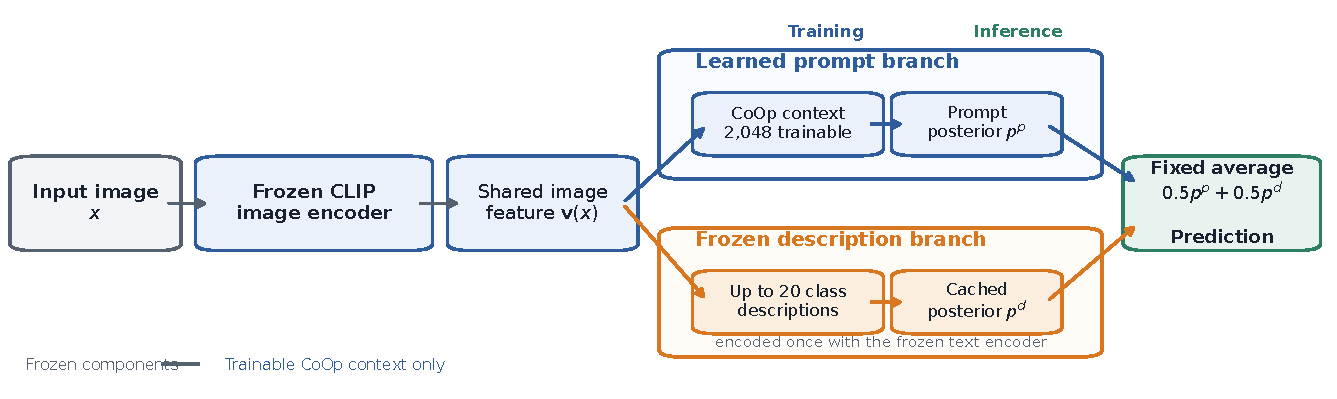
\includegraphics[width=0.98\textwidth]{图1-方法框架.pdf}
\caption{Overview of TextConsistency. A frozen CLIP image representation is scored against a learned CoOp classifier and a cached class-description classifier. Only the CoOp context tokens are trained; the two independently normalised posteriors are averaged with a fixed coefficient of 0.5.}
\label{fig:method}
\end{figure*}

\subsection{Parameter and Computation Cost}

Relative to CoOp, TextConsistency adds zero trainable parameters. In our ViT-B/16 implementation, CoOp trains 2,048 context parameters. The cached class-description tensor occupies 0.0977 MiB in the measured UCF101 setting. During inference, the extra operations are one image-to-prototype matrix multiplication, one softmax, and one probability average. No text encoding is performed in the timed inference loop.

\section{Experiments}
\label{sec:experiments}

\subsection{Datasets and Evaluation Protocol}

We evaluate on ten datasets from the standard base-to-novel benchmark: Caltech101, OxfordPets, StanfordCars, OxfordFlowers, Food101, FGVC Aircraft, SUN397, DTD, EuroSAT, and UCF101. They cover generic objects, fine-grained categories, food, aircraft, scenes, textures, remote sensing, and human actions. We use the public class splits associated with CoOp and CoCoOp \cite{zhou2022coop,zhou2022cocoop}. ImageNet is not included because a verified local run was unavailable; therefore all averages in this paper are explicitly ten-dataset averages.

For every trainable method, we use 16 shots per base class and random seeds 1, 2, and 3. We first average base and novel accuracy over seeds and then compute dataset-level HM using Eq.~\eqref{eq:hm}. Cross-dataset summaries are unweighted macro averages over the ten dataset-level values. Zero-shot CLIP has no training seed.

\subsection{Implementation Details}

All local experiments use OpenAI CLIP ViT-B/16. CoOp uses four context tokens, batch size 16, SGD with learning rate 0.002 and momentum 0.9, cosine scheduling, and 20 epochs. Images are resized to $224\times224$ with the CLIP normalisation. The description branch uses the deterministic filtering rule above, at most 20 stored descriptions per class, and the same frozen CLIP logit scale as the learned branch. Description embeddings are computed once and cached. The mixing coefficient is always 0.5.

The local CoCoOp baseline follows its standard recipe with four context tokens, batch size 1, and 10 epochs. It shares the backbone, shots, class splits, and three seeds with our evaluation, but its training budget is not identical to the 20-epoch CoOp recipe. We therefore treat it as a standard-recipe baseline rather than an equal-compute ablation.

\subsection{Baselines and Reporting Boundary}

The locally evaluated baselines are zero-shot CLIP, CoOp, and CoCoOp. Their results are separated from published numbers for CuPL, CoCoOp, KgCoOp, MaPLe, and PromptSRC \cite{pratt2023cupl,zhou2022cocoop,yao2023kgcoop,khattak2023maple,khattak2023promptsrc}. Published values are used only for positioning and are marked with $\dagger$; they are not claimed as local reproductions.

\section{Results}
\label{sec:results}

\subsection{Local Base-to-Novel Comparison}

\begin{table*}[t]
\centering
\caption{Matched harmonic-mean accuracy (\%) on the standard eleven base-to-novel benchmarks. Both methods use CLIP ViT-B/16, the official class splits, and the same three CoOp checkpoints per dataset.}
\label{tab:local_hm}
\scriptsize
\setlength{\tabcolsep}{3.2pt}
\resizebox{\textwidth}{!}{%
\begin{tabular}{lrrrrrrrrrrrr}
\toprule
Method & UCF & DTD & Air. & Euro. & Flw. & Cal. & Pets & Food & Cars & SUN & IN & Avg. \\
\midrule
CoOp & 74.42 & 63.79 & 34.26 & 67.52 & 81.07 & 95.95 & 96.39 & 90.51 & 72.35 & 77.05 & 72.39 & 75.06 \\
\textbf{TextConsistency} & 79.47 & 70.99 & 38.46 & 76.65 & 85.06 & 96.09 & 96.63 & 91.30 & 73.16 & 79.74 & 74.05 & \textbf{78.33} \\
\bottomrule
\end{tabular}%
}
\end{table*}

\begin{table}[t]
\centering
\caption{Eleven-dataset macro averages for the matched comparison (\%). HM is computed for each dataset before macro averaging.}
\label{tab:average_metrics}
\small
\begin{tabular}{lrrr}
\toprule
Method & Base & Novel & HM \\
\midrule
CoOp & 81.39 & 70.34 & 75.06 \\
\textbf{TextConsistency} & 81.13 & 76.00 & 78.33 \\
\bottomrule
\end{tabular}
\end{table}


Table~\ref{tab:local_hm} reports dataset-level HM. TextConsistency reaches 78.75 on average, compared with 71.88 for zero-shot CLIP, 75.33 for matched CoOp, and 76.15 for local CoCoOp. The gains are 3.42 percentage points over CoOp and 2.60 points over CoCoOp. TextConsistency exceeds local CoCoOp on all ten datasets.

Table~\ref{tab:average_metrics} separates base and novel accuracy. Relative to CoOp, TextConsistency changes the average base accuracy from 81.88 to 81.58 while improving novel accuracy from 70.50 to 76.44. The 5.94-point novel gain is therefore the main source of the improved balance. Relative to local CoCoOp, TextConsistency improves both the macro base and novel averages, although this comparison uses the standard training recipe of each method rather than equal epochs.

The improvement over CoOp is positive for every dataset and all 30 seed-level comparisons. It is largest on EuroSAT, DTD, UCF101, FGVC Aircraft, and OxfordFlowers. The gains on Caltech101, OxfordPets, Food101, and StanfordCars are smaller, which indicates that the frozen semantic branch is most useful when the learned prompt exhibits a larger base-novel gap.

Figure~\ref{fig:dataset-gains} visualises these dataset-level gains. The comparison with CoOp isolates the effect of adding the frozen description posterior to the matched learned prompt, whereas the comparison with CoCoOp positions the method against an independently trained conditional-prompt baseline. All bars remain above zero, but their range also shows that the benefit is dataset dependent rather than a uniform offset.

\begin{figure*}[t]
\centering
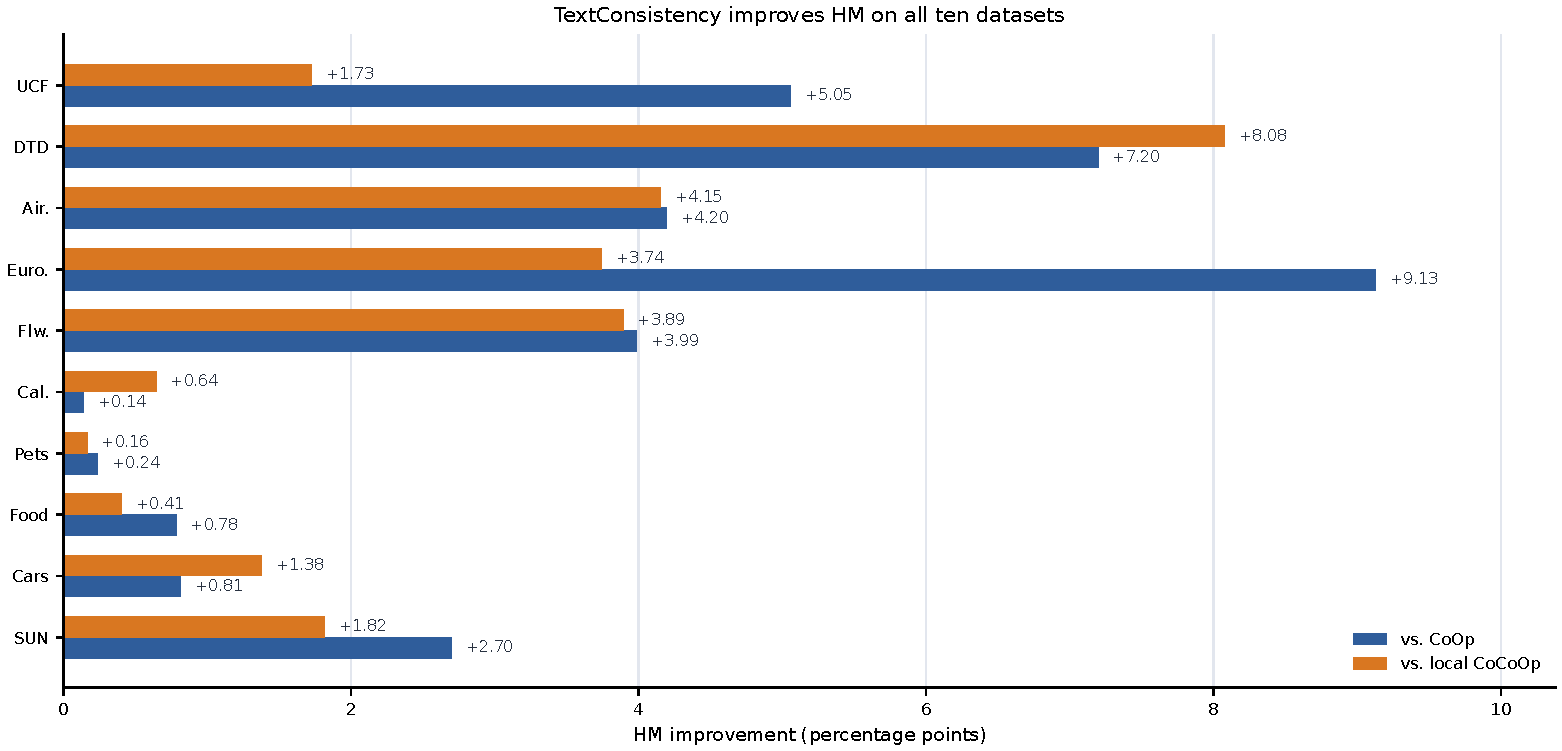
\includegraphics[width=0.92\textwidth]{图2-十数据集增益.pdf}
\caption{Per-dataset HM improvement of TextConsistency over matched CoOp and locally evaluated CoCoOp. Positive values indicate higher harmonic mean. All values are computed from the audited three-seed dataset summaries.}
\label{fig:dataset-gains}
\end{figure*}

\subsection{Comparison with Published Results}

\begin{table*}[t]
\centering
\caption{Comparison with published base-to-novel HM results on the ten datasets common to all methods. Published values are marked with $\dagger$ and are not local reproductions.}
\label{tab:published_hm}
\scriptsize
\setlength{\tabcolsep}{3.2pt}
\resizebox{\textwidth}{!}{%
\begin{tabular}{lrrrrrrrrrrr}
\toprule
Method & UCF & DTD & Air. & Euro. & Flw. & Cal. & Pets & Food & Cars & SUN & Avg. \\
\midrule
CuPL$^\dagger$ & 76.40 & 61.30 & 33.20 & 61.80 & 76.10 & 95.60 & 95.80 & 90.60 & 68.80 & 75.70 & 73.53 \\
CoCoOp$^\dagger$ & 77.64 & 64.85 & 27.74 & 71.21 & 81.71 & 95.84 & 96.43 & 90.99 & 72.01 & 78.27 & 75.67 \\
KgCoOp$^\dagger$ & 79.65 & 64.35 & 34.83 & 73.48 & 83.65 & 96.03 & 96.18 & 91.09 & 73.36 & 78.36 & 77.10 \\
MaPLe$^\dagger$ & 80.77 & 68.16 & 36.50 & 82.35 & 82.56 & 96.02 & 96.58 & 91.38 & 73.47 & 79.75 & 78.75 \\
PromptSRC$^\dagger$ & 82.74 & 71.75 & 40.15 & 82.32 & 85.95 & 96.02 & 96.30 & 91.10 & 76.58 & 80.52 & 80.34 \\
\textbf{TextConsistency} & 79.47 & 70.99 & 38.46 & 76.65 & 85.06 & 96.09 & 96.63 & 91.30 & 73.16 & 79.74 & \textbf{78.75} \\
\bottomrule
\end{tabular}%
}
\end{table*}


Table~\ref{tab:published_hm} recomputes a ten-dataset average using the datasets common to all listed methods. TextConsistency is 5.22 points above CuPL, 3.09 points above the published CoCoOp values, and 1.66 points above KgCoOp. Its 78.75 average is effectively tied with MaPLe at the reported precision and is 1.59 points below PromptSRC. Because these are paper-reported values from different implementations, the table should be interpreted as positioning rather than a controlled ranking. In particular, the result does not support a state-of-the-art claim.

\subsection{Component Analysis}
\label{sec:component}

\begin{table*}[t]
\centering
\caption{Component comparison using HM (\%). The description branch is frozen. Both fusion variants use a fixed weight of 0.5.}
\label{tab:components}
\scriptsize
\setlength{\tabcolsep}{3.2pt}
\resizebox{\textwidth}{!}{%
\begin{tabular}{lrrrrrrrrrrr}
\toprule
Method & UCF & DTD & Air. & Euro. & Flw. & Cal. & Pets & Food & Cars & SUN & Avg. \\
\midrule
CoOp & 74.42 & 63.79 & 34.26 & 67.52 & 81.07 & 95.95 & 96.39 & 90.51 & 72.35 & 77.05 & 75.33 \\
Description only & 76.46 & 63.30 & 34.83 & 69.99 & 76.69 & 96.29 & 95.27 & 90.58 & 67.53 & 76.73 & 74.77 \\
Logit fusion & 78.76 & 70.75 & 38.31 & 75.69 & 83.73 & 96.09 & 96.64 & 91.30 & 72.86 & 79.54 & 78.37 \\
\textbf{Probability fusion} & 79.47 & 70.99 & 38.46 & 76.65 & 85.06 & 96.09 & 96.63 & 91.30 & 73.16 & 79.74 & \textbf{78.75} \\
\bottomrule
\end{tabular}%
}
\end{table*}


The description-only branch obtains 74.77 average HM, below CoOp at 75.33. Its value lies in complementarity rather than standalone strength. Fixed logit fusion raises the average to 78.37, showing that combining the two semantic sources is already effective. Probability fusion further raises it to 78.75 and is the final method. The same coefficient is used for every dataset; the difference is not produced by dataset-specific weight selection.

The description branch is deterministic for a fixed dataset and split. Repeating it alongside three CoOp checkpoints does not constitute three independent description-model trainings. Our statistical unit for the trainable branch remains the three CoOp seeds.

\subsection{Class-name Control and Global Fusion Weight}
\label{sec:semantic_control}

\begin{table}[t]
\centering
\caption{Class-name control on all eleven datasets with matched frozen checkpoints. All values are three-seed macro averages (\%).}
\label{tab:class_name_control}
\small
\setlength{\tabcolsep}{7pt}
\begin{tabular}{lrrr}
\toprule
Method & Base & Novel & HM \\
\midrule
CoOp & 81.39 & 70.34 & 75.06 \\
Class name only & 69.49 & 74.31 & 71.71 \\
CoOp + class name & 80.71 & 73.80 & 76.84 \\
Description only & 72.01 & 77.78 & 74.59 \\
\textbf{TextConsistency} & \textbf{81.13} & \textbf{76.00} & \textbf{78.33} \\
\bottomrule
\end{tabular}
\end{table}


Table~\ref{tab:class_name_control} uses all ten main-study datasets and the exact matched checkpoints from the primary evaluation. Relative to the same CoOp checkpoints fused with ordinary class-name prompts, TextConsistency improves macro HM from 77.23 to 78.75, a gain of 1.53 points. It is higher on nine of ten datasets and 25 of 30 matched dataset-seed comparisons. The largest gain is 6.18 points on EuroSAT; the newly completed DTD and FGVC Aircraft controls add 3.38 and 2.69 points, respectively, while StanfordCars is 0.18 points lower. The result therefore supports an average contribution from descriptive semantics without implying uniform improvement on every dataset.

\begin{figure*}[t]
\centering
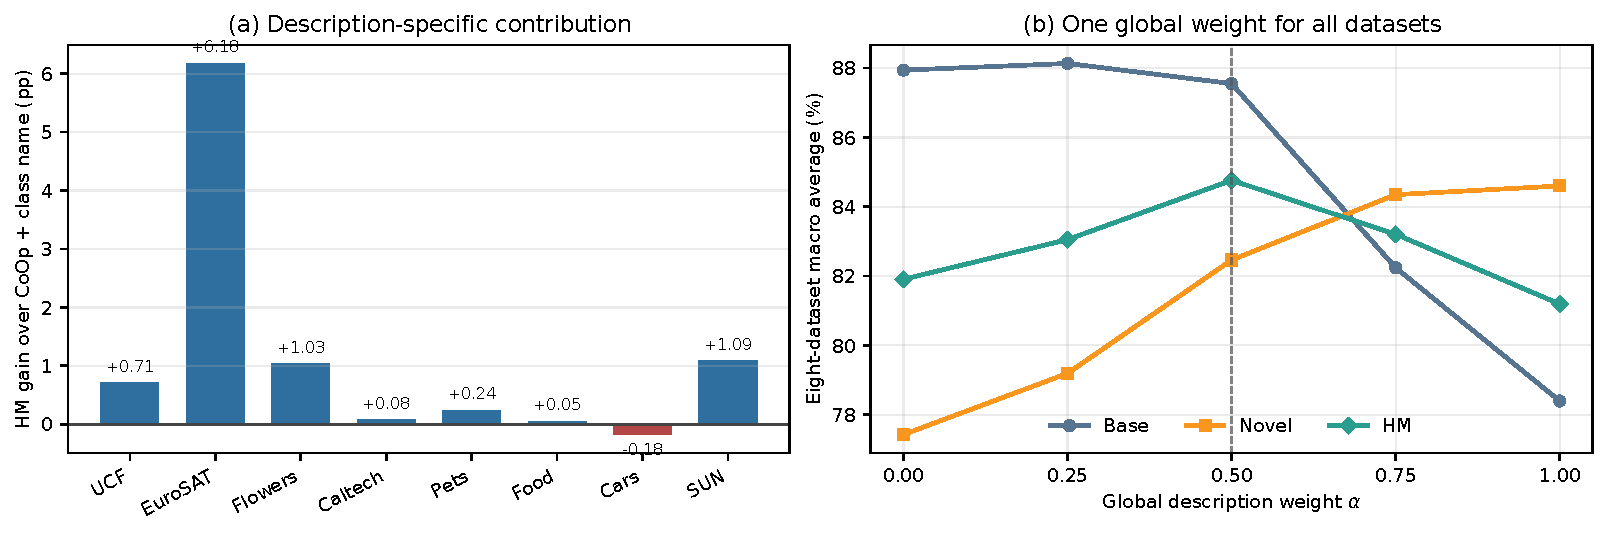
\includegraphics[width=0.98\textwidth]{图4-语义对照与权重稳健性.pdf}
\caption{Controlled semantic and weight analyses on all ten datasets. (a) HM difference between TextConsistency and an otherwise matched CoOp-plus-class-name probability average. (b) Base, novel, and HM macro averages for one global description weight shared by every dataset. The main method remains the pre-specified $\alpha=0.5$.}
\label{fig:semantic_control}
\end{figure*}

Figure~\ref{fig:semantic_control}(b) reports the common grid $\alpha\in\{0,0.25,0.5,0.75,1\}$ without selecting a dataset-specific value. The pre-specified midpoint obtains the highest macro HM, 78.75. Both intermediate mixtures outperform the two single-branch endpoints, while increasing $\alpha$ trades base accuracy for novel accuracy. This pattern is consistent with the intended balance between adaptation and frozen semantic coverage.

\subsection{Stability Across Seeds}

For each seed, we compare TextConsistency and CoOp using predictions from the same trained checkpoint. All 30 paired HM differences are positive. On the first five completed datasets, the mean paired gains were $+5.07$ on UCF101, $+7.19$ on DTD, $+4.20$ on FGVC Aircraft, $+9.88$ on EuroSAT, and $+4.01$ on OxfordFlowers. The remaining five datasets also produced three positive seed-level differences each. Because each dataset has only three seeds, we use these results as evidence of directional stability and do not make strong significance claims from small-sample confidence intervals.

Figure~\ref{fig:diagnostics} summarises the component, stability, and cost evidence in a common visual form. Panel (a) confirms that the description branch is complementary rather than independently dominant. Panel (b) retains every paired seed result and exposes the much smaller gains on already saturated datasets. Panel (c) places the 3.42-point macro-HM improvement next to the measured 0.74\% batch-64 latency increase; the axes combine different evaluation scopes and are intended as a compact accuracy-cost summary rather than a hardware-independent frontier.

\begin{figure*}[t]
\centering
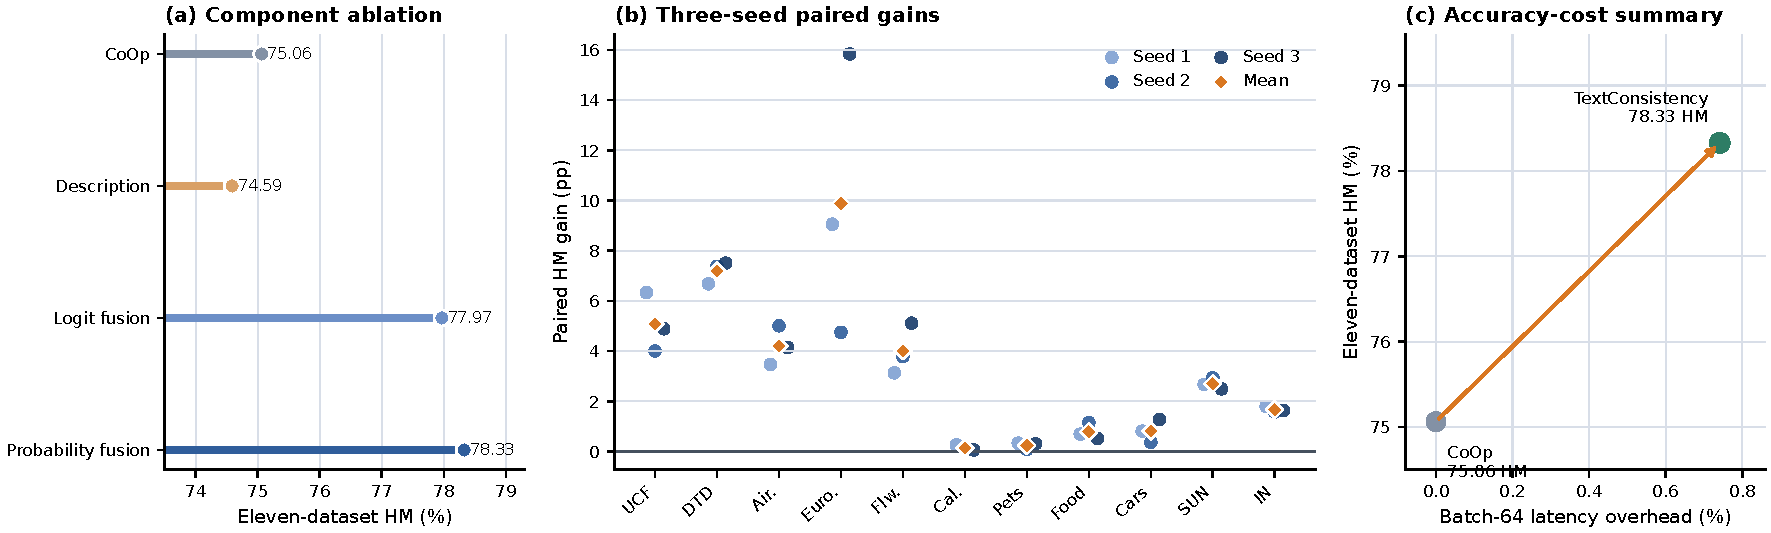
\includegraphics[width=0.99\textwidth]{图3-消融稳定性效率.pdf}
\caption{Diagnostic summary. (a) Ten-dataset component HM. (b) Paired TextConsistency-minus-CoOp HM gains for all three seeds on each dataset; diamonds denote dataset means. (c) Ten-dataset macro HM versus batch-64 latency overhead measured on the UCF101 novel split of one RTX 4090.}
\label{fig:diagnostics}
\end{figure*}

\subsection{Inference Efficiency}

\begin{table}[t]
\centering
\caption{Inference efficiency on one RTX 4090 using the UCF101 novel split. Text features are pre-computed.}
\label{tab:efficiency}
\small
\setlength{\tabcolsep}{4.5pt}
\begin{tabular}{lrrrr}
\toprule
Method & Batch & ms/batch & img/s & Extra latency \\
\midrule
CoOp & 1 & 18.827 & 53.12 & 0.00\% \\
TextConsistency & 1 & 18.904 & 52.90 & 0.41\% \\
CoOp & 64 & 90.128 & 710.10 & 0.00\% \\
TextConsistency & 64 & 90.796 & 704.88 & 0.74\% \\
\bottomrule
\end{tabular}
\end{table}


Table~\ref{tab:efficiency} reports CUDA-event measurements on one RTX 4090. Each setting uses 20 warm-up iterations followed by 100 timed iterations on the same UCF101 novel checkpoint and input tensors. At batch size 64, TextConsistency increases latency from 90.128 to 90.796 ms per batch, an overhead of 0.74\%. Incremental peak memory is unchanged at the allocator resolution used in this experiment. These measurements exclude model loading, disk I/O, CPU preprocessing, and one-time text encoding.

\section{Discussion and Limitations}
\label{sec:limitations}

The experiments support a narrow conclusion: a fixed posterior average can recover useful frozen semantics that CoOp underuses after base-class adaptation. They do not show that natural-language descriptions are universally superior to learned prompts. The description-only average is lower than CoOp, and the smallest fusion gains occur on datasets where the two branches are already similarly strong.

Several limitations remain. First, ImageNet is absent, so the ten-dataset average cannot be compared directly with the common eleven-dataset benchmark average. Second, the local CoCoOp baseline uses its standard 10-epoch recipe while CoOp and TextConsistency use 20 epochs. Third, the descriptions originate from the public CuPL/ProText assets; we do not compare alternative language models, generation instructions, or description budgets. Fourth, the global-weight analysis uses a coarse five-point grid and evaluates the same datasets as the main study; it does not establish calibration robustness under an external distribution shift. Finally, the efficiency result is measured on one GPU and should not be treated as a hardware-independent latency guarantee.

The full experimental evidence was accumulated in audited batches with frozen data splits, seeds, source hashes, checkpoints, raw predictions, and independent recomputation. This makes the reported values traceable, although a future single-release rerun including ImageNet would provide a cleaner eleven-dataset benchmark package.

\section{Conclusion}

We presented TextConsistency, a parameter-free extension to CoOp that averages the class probabilities from learned prompts and frozen class descriptions. The method keeps CLIP frozen, leaves prompt training unchanged, uses a single fixed fusion coefficient, and caches the description prototypes. Across ten base-to-novel datasets, it improves average HM from 75.33 to 78.75 over matched CoOp and exceeds locally evaluated CoCoOp on every dataset. Component results show that the benefit comes from combining complementary branches, and an RTX 4090 measurement shows less than one percent batch-64 latency overhead. The current evidence supports TextConsistency as a simple and reproducible method for improving novel-class balance, while ImageNet evaluation and broader description-generation studies remain future work.

\section*{Data and Code Availability}

The implementation, frozen configurations, result tables, audit scripts, and experiment summaries are available in the \href{https://github.com/guiyangyuan/textconsistency_v2_tune}{public GitHub repository}. The release separates local reproductions from published comparison values and includes machine-readable CSV and JSON summaries. The description files are traced to fixed ProText and CuPL commits; their hashes, the two local text clean-ups, and the upstream licence locations are recorded in the repository's preparation reports.

\bibliographystyle{elsarticle-num}
\bibliography{cas-refs}

\end{document}
